%===================================== CHAP 2 =================================

\chapter{Background}
\label{chp:background}


\section{Evolution}
\label{sec:evolution}

In nature, evolution is the process governing change and preservation of
hereditary traits in populations of biological organisms. It allows species to
adapt to their environment over generations through reproduction, variation and
survival of the fittest \cite{Darwin1859}.

Artificial evolution seeks to harness the powerful adaptive capabilities of
natural evolution and apply them to general problem solving and learning. While
research on the subject has branched into many different sub-areas, the general
concept of optimizing a population of individuals with respect to some fitness
function using mechanisms inspired by natural evolution, is referred to using
the umbrella term Evolutionary Computation (EC) \cite{Back1997}.

One of the greatest strengths of EC is how universally applicable it is.
Evolutionary algorithms have successfully been applied to many different problem
domains, such as robotics \cite{Floreano2000}, bioinformatics
\cite{KosakovskyPond2006}, medicine \cite{Fitzgerald:2015:IAS:2739480.2754761}
and many more.

\subsection{Genetic Algorithm}

The most common type of EA is the Genetic Algorithm (GA)
\cite{Goldberg:1989:GAS:534133}. GAs use, as shown in \ref{fig:ga}, genetic
operators such as mutation, crossover and selection to evolve a population of
potential solutions to a problem, subject to some fitness function. The fitness
function deems how fit an individual is, and thereby how likely it is to be
selected for reproduction. It is a measure of how well the indivual performs as
a solution to the problem at hand. The algorithm continues until an individual
with a fitness higher than some predetermined threshold is found. Individuals
are represented as genomes, commonly with a genotype encoded as a bitstring
which serves as a blueprint to create the solution, the phenotype.

\begin{figure}[ht]
  \centering
  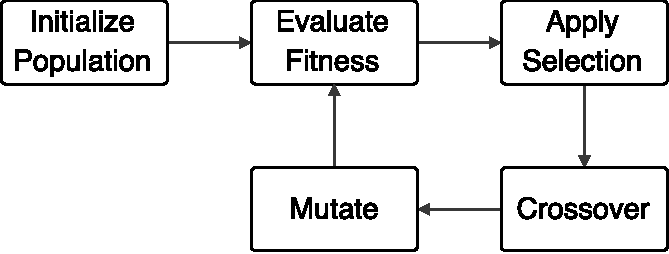
\includegraphics[width=0.5\linewidth]{fig/ga}
  \caption{Genetic Algorithm process.}
  \label{fig:ga}
\end{figure}

\subsection{Genetic Programming}

Genetic Programming (GP), introduced by John Koza \cite{Koza:1992:GPP:138936},
is a technique attempting to automate the programming of computers. This is done
by evolving a population of programs whose fitness is evaluated by executing
them and comparing to the desired results. Programs are encoded in genotypes as
tree structures, as opposed to as binary strings. This allows crossover and
mutation operators to be implemented in such away that the resulting programs
are structurally sound.


\section{Development}
\label{sec:development}

Biological development is the natural process that allows complex multi-cellular
organisms to be built starting from a single cell using instructions encoded in
the DNA of the organism. The most easily recognizable example is the development
of humans from a single cell, the zygote, containing the combined genetic
material of the parents, through cell division and differentiation. The human
genome does not contain an exhaustive description and blueprint of each
individual human. Rather, it consists of instructions governing how cells should
divide and differentiate based on their surrounding cells and feedback from the
environment.

Developmental processes in nature have many properties that make them desireable
to mimic through artificial development. For instance, the number of cells in
the human body is orders of magnitudes larger than the amount of information
encoded in our DNA \cite{Bianconi2013}. In general, the performance of GAs and
GP implementations decline as the size of the genome increases, as mutations are
more likely to be detrimental with regards to fitness. By introducing
development as an indirect mapping between genotype and phenotype, programs and
structures that scale to arbitrary dimensions can be produced while still
maintaining a search space that the EA method in question can efficiently
explore. Systems that combine evolution and development in this way are often
referred to as EvoDevo systems \cite{Hall2003}.

Where evolution allows a species to adapt over the span of generations,
development is an ongoing process throughout the lifetime of each individual,
allowing for adaption based on changes to the environment \cite{Tufte2008}. This makes EvoDevo
particularily well suited in the design of robust and adaptive artificial
intelligence agents.

\section{Cellular Computing}
\label{sec:cellular-computing}

Most computing devices in use today have been developed on the foundation of the
von Neumann architecture \cite{VonNeumann1993}, a single complex processor
performing one complex task at a time. Recently, the field of cellular computing
has seen growing interest. Cellular computing, as described by Sipper in
\cite{Sipper1999}, is built on three principles: simplicity, vast parallelism
and locality. It seeks to exploit emergent computational capabilities between
large numbers of locally connected simple cells. Sipper presents cellular
computing as an abstract framework, within which many variations of the paradigm
can exist based on a number of properties. These include cell type (which types
of values a cell can take; discrete or continuous), cell definition (how the
behavior of cells is specified), cell mobility (wether or not cells can move
within their environment), cell connectivity (how cells are connected to
eachother; regular grid, (un)directed graph), topology of underlying environment
(if any), connection lines (what information to transmit between connected
cells), temporal dynamics (asynchronous vs. synchronous updating schemes),
uniformity (in cell type and connectivity) and determinism. Some well known
examples of paradigms that fit within the framework of cellular computing are
Random Boolean Networks (RBNs) and Cellular Automata (CAs).

\subsection{Cellular Automata}

The most well known example of cellular computing is the Cellular Automaton
(CA). Consisting of cells connected in a regular grid that transition between
discrete states based on the states of the cells in their neighborhood
\footnote{The von Neumann-neighborhood, consisting of cells directly north,
east, south and west of a cell, is a common choice.}. While each cell is not
capable of much on their own, the behavior emerging from interactions between
cells can give rise to complex dynamics. \figurename~\ref{fig:ca-example} shows
the behavior over eight timesteps of a simple, 1-dimensional, uniform CA
starting from a single cell, with each time-step shown on a new line. The rule
governing state transitions is shown in the boxes to the right in the figure.
Each box gives the neighborhood conditions on the top row and the resulting
state on the bottom.


\begin{figure}[ht]
  \centering
  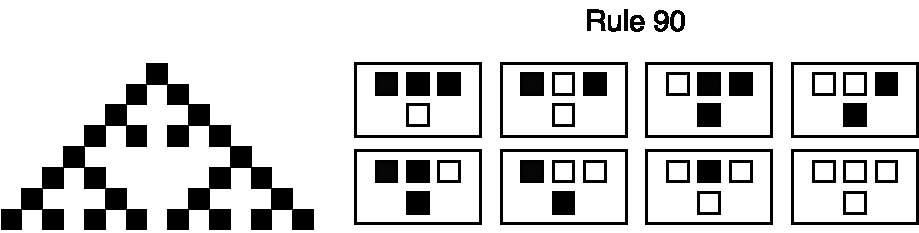
\includegraphics[width=0.6\linewidth]{fig/ca-example}
  \caption{
    Eight timesteps for a uniform 1-dimensional CA. The boxes to the right show
    the rule with which the cells are configured, Rule 90.
  }
  \label{fig:ca-example}
\end{figure}

Research into the computational capabilities of CAs can be said to have started
in the 1940s, with John von Neumann and Stanislaw Ulam designing a 2D CA capable
of self-reproduction \cite{Sipper1999}. Moving forward, the dynamics and
behavior of specific CA rules was examined in detail. For instance, the rule
used in Game of Life, introduced by mathematician John Conway in 1982, was
proven to be capable of universal computation \cite{Connelly1986}. Stephen
Wolfram shifted focus from studying specific rules, to investigating
characteristics of groups of rules, resulting in his classification of the CA
rulespace:

\begin{enumerate}
  \item Rules leading to homogenous state for all cells. Regardless of the
    initial configuration of the cells, they all converge to the same state
    after a transient period.
  \item Rules leading to stable or periodic structures.
  \item Rules leading to chaotic patterns.
  \item Rules leading to complex, long-lived structures. This is the only class
    that contains non-trivial automata.
\end{enumerate}

Wolfram proposed that the rules capable of universal computation, such as Game
of Life, reside in Class 4.

\begin{equation}
  \label{eqn:lambda}
  \lambda = 1 - \frac{q}{tot}
\end{equation}

Like Wolfram, Christopher Langton has performed quantitative and qualitative
studies of the CA rulespace \cite{Langton1990}. He hypothesized that it is more
likely to find rules capable of complex computational behavior in regions of the
rulespace where there is a phase transition between ordered and chaotic
dynamics. He introduced the $\lambda$-parameter as a measure of heterogeneity
for a rule. It is calculated, as shown in \ref{eqn:lambda}, where $q$ is the
number of transitions in a rule that lead to a chosen quiescent, or dead, state,
and $tot$ is the total number of transitions. For a CA with $N$ possible states
and a neighborhood-size of $K$, the total number of transitions is $K^N$. A
$\lambda$-value of $0$ indicates an entirely homogenous rule, where all possible
neighborhood configurations result in a transition to the quiescent state.
Maximally heterogenous rules will have a $\lambda$ of $1-1/N$.
\figurename~\ref{fig:ca-classes} shows how Wolframs 4 classes map onto Langtons
$\lambda$-space, with Class 4 coinciding with phase transition between ordered
and chaos behavior, the so called Edge of Chaos.

\begin{figure}[ht]
  \centering
  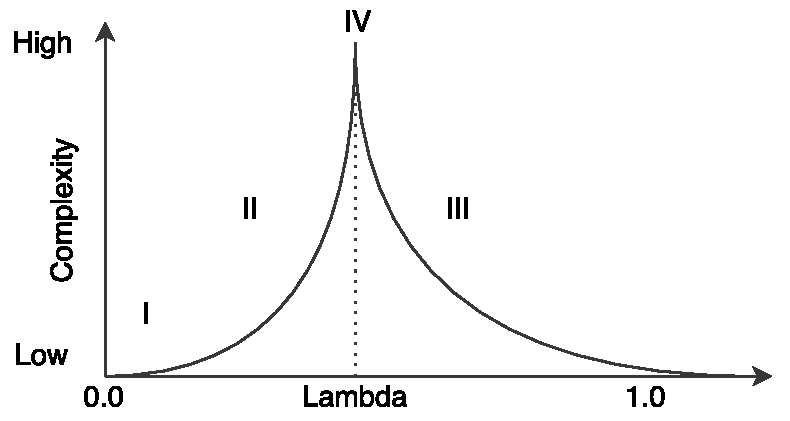
\includegraphics[width=0.5\linewidth]{fig/ca-classes}
  \caption{Wolframs rule classes mapped onto Langtons $\lambda$-space.}
  \label{fig:ca-classes}
\end{figure}


\subsection{Developmental Cellular Architectures}

One of the major challenges faced by cellular computing systems is how to
program one. Manually programming the functionality and connectivity of each
cell to achieve the desired emergent properties is both exceptionally
time-consuming and hard to do when the problem to be solved involves global
coordination. Sipper proposes to automate the programming of cellular systems
through an adaptive process such as an EA. In \cite{Mitchell1993}, Mitchell et
al. use a GA to evolve CA rules for solving problems requiring global
coordination. Each individual is a bitstring representing the next-states for
all possible neighborhood configurations. With a neighborhood size of 7, each
genome is $2^7=128$ bits long yielding a search space size of $2^{128}$. The
authors are able to successfully evolve CAs that solve the problems for which
they where created.

A different approach is taken by Sipper \cite{Sipper2004} in order to evolve
non-uniform CAs. Where Mitchell et al. evolve a population of rules, doing this
for a non-uniform CA would require an exceptionally large genome in order to
specify the rule for each cell, increasing the search space exponentially,
making it infeasible to search through using a standard GA. Sipper instead
works with a single CA initialized with a random rule in each cell. The fitness
of each cell is accumulated over some number of simulations of the CA starting
from different initial state configurations, after which evolutionary mechanisms
are applied in a local manner, between connected cells. Through this method,
Sipper is able to evolve non-uniform CAs that outperform the uniform ones
evolved by Mitchell et al. on the same tasks.


\tikzstyle{block} = [draw, fill=white!20, rectangle, 
    minimum height=2em, minimum width=5em]
\tikzstyle{sum} = [draw, fill=blue!20, circle, node distance=1cm]
\tikzstyle{input} = [coordinate]
\tikzstyle{output} = [coordinate]
\tikzstyle{pinstyle} = [pin edge={to-,thin,black}]
\begin{figure}[ht]
  \begin{adjustbox}{max size={\textwidth}}
  \begin{tikzpicture}
  [help lines/.style={draw=black},
  every node/.style={help lines,rectangle,minimum size=3mm},
  cellular automaton/.style={draw=none,row sep=0mm,column sep=0mm, ampersand replacement=\&, label=above:#1},
  cellular automaton2/.style={draw=none,row sep=0mm,column sep=0mm, ampersand replacement=\&, label=below:#1},
  w/.style={fill=white,help lines},
  b/.style={fill=black, help lines},
  r/.style={fill=red, help lines},
  g/.style={fill=black!30!green,help lines}]

    \matrix (DS0) [cellular automaton={DS 0}] {
      \node[w] {};\& \node[w] {};\& \node[w] {};\& \node[w] {};\& \node[w] {}; \\
      \node[w] {};\& \node[w] {};\& \node[w] {};\& \node[w] {};\& \node[w] {}; \\
      \node[w] {};\& \node[w] {};\& \node[g] {};\& \node[w] {};\& \node[w] {}; \\
      \node[w] {};\& \node[w] {};\& \node[w] {};\& \node[w] {};\& \node[w] {}; \\
      \node[w] {};\& \node[w] {};\& \node[w] {};\& \node[w] {};\& \node[w] {}; \\
    };
    \matrix (DS1) [cellular automaton={DS 1}, right=of DS0] {
      \node[w] {};\& \node[w] {};\& \node[w] {};\& \node[w] {};\& \node[w] {}; \\
      \node[w] {};\& \node[w] {};\& \node[g] {};\& \node[w] {};\& \node[w] {}; \\
      \node[w] {};\& \node[g] {};\& \node[g] {};\& \node[g] {};\& \node[w] {}; \\
      \node[w] {};\& \node[w] {};\& \node[r] {};\& \node[w] {};\& \node[w] {}; \\
      \node[w] {};\& \node[w] {};\& \node[w] {};\& \node[w] {};\& \node[w] {}; \\
    };
    \matrix (SS0) [cellular automaton2={SS 0}, below left=of DS1] {
      \node[w] {};\& \node[b] {};\& \node[w] {};\& \node[w] {};\& \node[b] {}; \\
      \node[b] {};\& \node[w] {};\& \node[w] {};\& \node[w] {};\& \node[w] {}; \\
      \node[w] {};\& \node[w] {};\& \node[b] {};\& \node[b] {};\& \node[w] {}; \\
      \node[w] {};\& \node[b] {};\& \node[w] {};\& \node[w] {};\& \node[w] {}; \\
      \node[w] {};\& \node[b] {};\& \node[b] {};\& \node[w] {};\& \node[b] {}; \\
    };
    \matrix (SS1) [cellular automaton2={SS 1}, right=of SS0] {
      \node[w] {};\& \node[b] {};\& \node[w] {};\& \node[w] {};\& \node[b] {}; \\
      \node[b] {};\& \node[w] {};\& \node[b] {};\& \node[w] {};\& \node[w] {}; \\
      \node[w] {};\& \node[b] {};\& \node[w] {};\& \node[b] {};\& \node[w] {}; \\
      \node[w] {};\& \node[b] {};\& \node[w] {};\& \node[w] {};\& \node[w] {}; \\
      \node[w] {};\& \node[b] {};\& \node[b] {};\& \node[w] {};\& \node[b] {}; \\
    };
    \matrix (SSN) [cellular automaton2={SS N}, right=of SS1] {
      \node[w] {};\& \node[b] {};\& \node[w] {};\& \node[w] {};\& \node[b] {}; \\
      \node[b] {};\& \node[w] {};\& \node[w] {};\& \node[w] {};\& \node[w] {}; \\
      \node[w] {};\& \node[w] {};\& \node[b] {};\& \node[w] {};\& \node[w] {}; \\
      \node[w] {};\& \node[b] {};\& \node[w] {};\& \node[w] {};\& \node[w] {}; \\
      \node[w] {};\& \node[b] {};\& \node[b] {};\& \node[w] {};\& \node[b] {}; \\
    };
    \matrix (SS01) [cellular automaton2={SS 0}, right=of SSN] {
      \node[w] {};\& \node[b] {};\& \node[w] {};\& \node[w] {};\& \node[b] {}; \\
      \node[b] {};\& \node[w] {};\& \node[w] {};\& \node[w] {};\& \node[w] {}; \\
      \node[w] {};\& \node[w] {};\& \node[b] {};\& \node[w] {};\& \node[w] {}; \\
      \node[w] {};\& \node[b] {};\& \node[w] {};\& \node[w] {};\& \node[w] {}; \\
      \node[w] {};\& \node[b] {};\& \node[b] {};\& \node[w] {};\& \node[b] {}; \\
    };
    \matrix (SS11) [cellular automaton2={SS 1}, right=of SS01] {
      \node[w] {};\& \node[b] {};\& \node[b] {};\& \node[w] {};\& \node[b] {}; \\
      \node[b] {};\& \node[w] {};\& \node[b] {};\& \node[w] {};\& \node[w] {}; \\
      \node[b] {};\& \node[b] {};\& \node[w] {};\& \node[b] {};\& \node[w] {}; \\
      \node[w] {};\& \node[b] {};\& \node[w] {};\& \node[w] {};\& \node[w] {}; \\
      \node[w] {};\& \node[b] {};\& \node[w] {};\& \node[w] {};\& \node[b] {}; \\
    };
    \matrix (SSN1) [cellular automaton2={SS N}, right=of SS11] {
      \node[w] {};\& \node[b] {};\& \node[w] {};\& \node[w] {};\& \node[b] {}; \\
      \node[b] {};\& \node[w] {};\& \node[b] {};\& \node[w] {};\& \node[w] {}; \\
      \node[w] {};\& \node[w] {};\& \node[w] {};\& \node[w] {};\& \node[b] {}; \\
      \node[w] {};\& \node[b] {};\& \node[b] {};\& \node[w] {};\& \node[w] {}; \\
      \node[w] {};\& \node[b] {};\& \node[b] {};\& \node[w] {};\& \node[b] {}; \\
    };
    \matrix (DS2) [cellular automaton={DS 2}, above=of SS11] {
      \node[w] {};\& \node[w] {};\& \node[g] {};\& \node[w] {};\& \node[w] {}; \\
      \node[w] {};\& \node[w] {};\& \node[g] {};\& \node[w] {};\& \node[w] {}; \\
      \node[g] {};\& \node[g] {};\& \node[g] {};\& \node[g] {};\& \node[g] {}; \\
      \node[w] {};\& \node[w] {};\& \node[r] {};\& \node[w] {};\& \node[w] {}; \\
      \node[w] {};\& \node[w] {};\& \node[g] {};\& \node[w] {};\& \node[w] {}; \\
    };

    \node[draw=none] at ($(SS1)!.5!(SSN)$) {\ldots};
    \node[draw=none] at ($(SS11)!.5!(SSN1)$) {\ldots};

    \draw[->] (DS0) -- (DS1);
    \draw[->] (DS1) -- (DS2);
    \draw[->] (SS0) -- (SS1);
    \draw[->] (SS01) -- (SS11);
    \draw[black] (DS1.south west) -- (SS0.north west);
    \draw[black] (DS1.south east) -- (SSN.north east);
    \draw[black] (DS2.south west) -- (SS01.north west);
    \draw[black] (DS2.south east) -- (SSN1.north east);
    \draw[thick, ->] (2, 2) -- (12,2) node[midway, above, draw=none] {Time};
  \end{tikzpicture}
  \end{adjustbox}
  \caption{
    Development starting from a single green cell using the growth
    rule in Figure~\ref{fig:growth-rules}.
  }\label{fig:dev-example}
\end{figure}

\begin{figure}[ht]
  \centering
  \begin{tikzpicture}[g/.style={draw, minimum size=3mm,   
        fill=black!30!green},w/.style={draw, minimum size=3mm},r/.style={draw, minimum size=3mm, fill=red},
      m/.style={matrix of nodes, column sep=1pt, row sep=1pt, draw, label=below:#1}, node distance=1pt]

    \matrix (A) [m={Gw}]{
      &|[w]|\\
      |[w]|&|[w]|&|[g]|\\
      &|[w]|\\
    };
    \matrix (B) [m={Gn}, right=of A]{
      &|[w]|\\
      |[w]|&|[w]|&|[w]|\\
      &|[g]|\\
    };
    \matrix (C) [m={Ge}, right=of B]{
      &|[w]|\\
      |[g]|&|[w]|&|[w]|\\
      &|[w]|\\
    };
    \matrix (D) [m={Gs1}, right=of C]{
      &|[g]|\\
      |[w]|&|[r]|&|[w]|\\
      &|[w]|\\
    };
    \matrix (E) [m={Gs2}, right=of D]{
      &|[r]|\\
      |[w]|&|[g]|&|[w]|\\
      &|[w]|\\
    };
  \end{tikzpicture}
  \caption{
    Growth rules for a cellular developmental system where cells are
    either empty or of the green type.
  }\label{fig:growth-rules}

\end{figure}

A third approach to the design of cellular computing systems is presented by
Haddow and Tufte in \cite{Tufte2005a}. The authors use a developmental model to
allow complex non-uniform CAs to grow from a single cell, as shown in
\figurename~\ref{fig:dev-example}. Development occurs in discrete time steps, so
called development steps (DS). Between each DS, a number of state steps (SS)
occur, simulating the behavior of the organism developed so far as a CA. The
rules governing the development process, the genome, take both cell type and
state into consideration when deciding how to proceed. This means that the
behavioral dynamics of the organism being developed regulates the developmental
process. This type of coevolution of both structure and functionality is often
referred to as dynamical systems with dynamical structure (DS)$^2$
\cite{Spicher04atopological}.

While the three approaches to programming of cellular computating systems
outlined above achieve positive results, the task is still hard. In the case
with the developmental approach taken by Tufte, creating developmental rules is
as difficult as manually specifying type and functionality for each cell.
Combining development with evolution is possible \cite{7008733}, but the genome
size needed to express all regulatory possibilities in the genome is so large
that the resulting size of the search space makes it hard for the EA to reliably
converge. There is in other words still a ways to go before programming of
cellular computing systems can be considered a solved problem.

Another challenge faced by such systems is how to formulate problems and
encode/decode their inputs and outputs. In the works by Sipper and Mitchell,
problem input is encoded as the initial state of the CA, and the output is
interpreted from the state of cells after a number of state steps. This approach
takes away from the generality of cellular systems, as an evolved/developed
system will only be able to work specifically for the problem and encoding
scheme it was initially designed around. Adapting a system to apply to different
problems or to slight variations in input encoding will almost always require it
to be developed from scratch.

\section{Reservoir Computing}
\label{sec:reservoir-computing}

Artificial Neural Networks (ANNs) are a commonly used computational model in
machine learning and bio-inspired computing. Simple, feed forward ANNs lend
themselves well to problems were data can be spatially correlated, such as
classification. Many real world problems however, are temporal in nature.
Recurrent neural networks (RNNs) have been shown to be powerful tools for
solving temporal problems such as stock market prediction~\cite{Lawrence2001},
learning context free/sensitive languages~\cite{Gers2001} and speech
synthesis~\cite{Wu2016}. Training RNNs is computationally expensive and often
requires application specific adaptions of generalized training algorithms in
order to reliably converge~\cite{Hammer2002}. Several techniques have been
proposed that circumvent problems related to training, such as Echo State
Networks~\cite{Jaeger2001} (ESNs), Liquid State Machines~\cite{Maass2002} (LSMs)
and Backpropagation Decorrelation learning~\cite{Steil2004}. These all share the
common feature of only training weights of the output layer of the network,
while leaving the hidden layers of the network untrained or simply subject to
weight scaling. In~\cite{Verstraeten2007}, Verstraeten et al.\ propose that
systems based on this idea should be unified under the term reservoir computing
(RC).

In general, reservoir computing as a term describes any computational system
where a dynamic reservoir is excited by input data and output is generated by
performing classification/regression over reservoir state.
Figure~\ref{fig:rc-system} shows the basic architecture of any reservoir
computing system. With its origins in research on various types of recurrent
neural networks and training thereof, the reservoir in RC systems is often
represented as an RNN~\cite{Verstraeten2007}. However, any dynamic system
capable of eventually forgetting past perturbations and of responding distinctly
to different perturbations, can in principle be used. Snyder et
al.~\cite{Snyder2013} investigate using Random Boolean Networks, Yilmaz uses
Cellular Automata~\cite{Yilmaz2014} and Fernando et al.\ use a bucket of
water~\cite{Fernando2003}.

\begin{figure}[ht]
  \centering
  \begin{tikzpicture}[auto, node distance=2cm,>=latex']
    \node [block] (input) {Input};
    \node [block, right of=input] (reservoir) {Reservoir};
    \node [block, right of=reservoir] (readout) {Readout};
    \node [block, below of=reservoir] (f) {$f(x)$};
    \node [output, right of=readout] (output) {};

    \draw [->] (input) -- (reservoir);
    \draw [->] (reservoir) -- (readout);
    \draw [->] (readout) -- node [name=out] {Output} (output);
    \draw [->] (out) |- (f);
    \draw [->] (f) -- (reservoir);
  \end{tikzpicture}
  \caption{Basic overview of an RC system.}
\label{fig:rc-system}
\end{figure}

As outlined in Section~\ref{sec:cellular-computing} cellular computing systems
are capable of complex, vast parallell computing. Combined with artificial
development they are also highly adaptive. In this thesis we combine reservoir
computing and developmental cellular automata in an attempt to provide a
framework allowing for easier use and development of cellular systems.
\figurename~\ref{fig:rc-dev-ca} shows how input data perturbs the behavioral
part of the reservoir, the emerging CA, and output is extracted by using the
readout layer to classify the dynamics in the CA. RC systems provide a layer of
abstraction between I/O encoding/decoding and the computation occurring in the
CA. With this approach the goal of development and evolution is not to create a
CA configuration that is able to solve a specific problem under specific I/O
conditions, but rather to develop CAs with strong general computation
capabilities and strong ability to adapt to different input perturbations. A CA
that is general enough, could be used in many different contexts simply by
swapping out the readout layer.

\begin{figure}[ht]
  \centering
  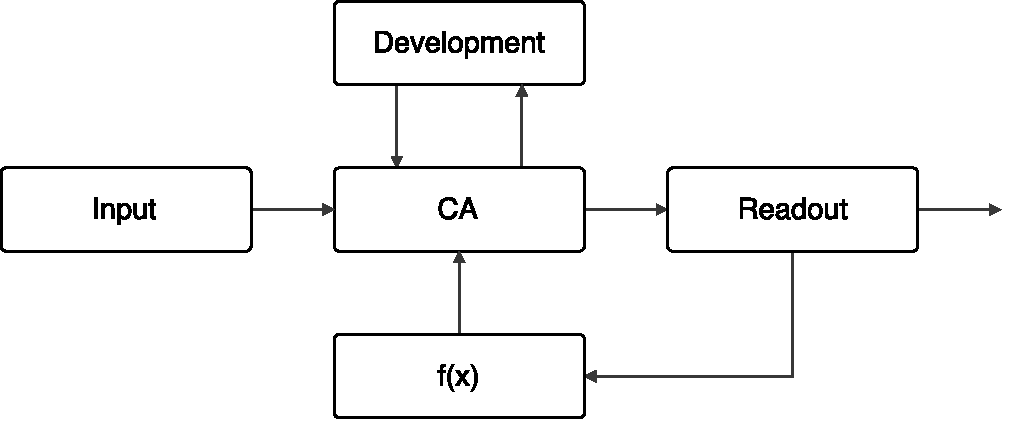
\includegraphics[width=0.6\linewidth]{fig/rc-dev-ca}
  \caption{RC system with developmental cellular reservoir.}
  \label{fig:rc-dev-ca}
\end{figure}

\subsection{Spiking Neural Networks as Readout Layers}

Artificial neural networks can be grouped into three generations, based on the
characteristics of their base computational unit, the neuron. The first
generation, based on McCulloch-Pitts neurons~\cite{McCulloch1943}, simple
threshold gates, allows for universal computation on digital input/output
values. In the second generation, neurons apply a non-linear, continuous
activation function on the weighted sum of their inputs.

The third generation of networks bases itself on spiking neurons, which model
the interaction between biological neurons more closely. In this model, a neuron
$v$ fires when its potential $P_v$ exceeds a threshold $\theta_v$. The potential
is, at any time, the sum of the postsynaptic potentials, resulting from firing
of presynaptic neurons. The contribution of a spike from presynaptic neuron $u$
at time $s$ to the potential $P_v$ of postsynaptic neuron $v$ is given by
$w_{u,v} \cdot \varepsilon_{u,v}(t-s)$, where $w_{u,v}$ is a weight representing
the strength of the synapse connecting $u$ and $v$, and $\epsilon_{u,v}(t-s)$
models the response of the spike as a function of time passed since the spike
occurred. A synapse can be both excitatory and inhibitory, meaning that its
contribution to the total potential $P_v$ can be both positive and negative. A
biologically plausible response function is shown in
figure~\ref{fig:response-function-snn}. From a machine learning perspective, the
trainable part of a spiking neural network, is the weight $w_{u,v}$, determining
to what degree spikes from a neuron $u$ influences the potential of neuron $v$.

\begin{figure}[ht]
  \centering
  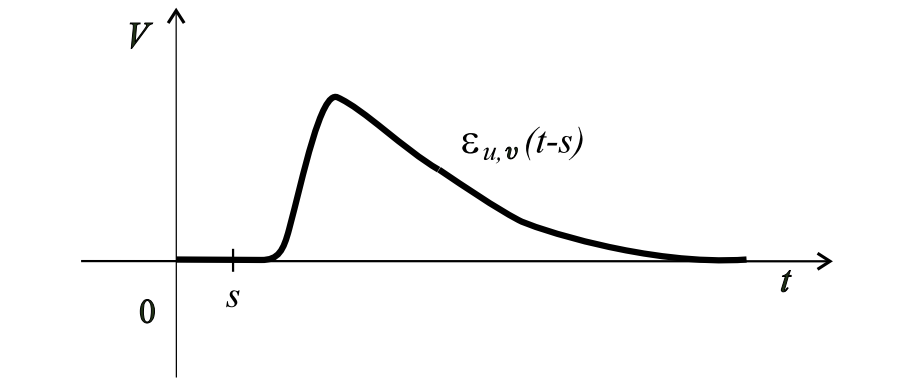
\includegraphics[width=0.5\linewidth]{fig/response-function-snn}
  \caption{Common spike response function shape, figure taken from \cite{Maass1997}.}
  \label{fig:response-function-snn}
\end{figure}


Spiking Neural Networks (SNNs) are of particular interest in the context of a cellular
RC system, where the reservoir dynamics are spiking in nature (i.e. a cell can
be either alive or dead). By using a spiking neural network as a readout layer,
data can flow through the RC-system as spikes from end to end. In the
specialization project leading up to this thesis, experiments to examine the
viability of SNNs as readout layers in RC system were carried out with successful
results (see Appendix~\ref{app:spec-proj-report}).


\section{Related Work}
\label{sec:related-work}

\subsection{IBM Truenorth}
\label{sec:truenorth}

The IBM Truenorth is a modular, non-von Neumann, ultra-low power computer
simulating a massive network of biologically plausible spiking
neurons~\footnote{\url{http://www.research.ibm.com/articles/brain-chip.shtml}}.
It consists of 4096 neurosynaptic cores, each simulating 256 neurons and
$256\times256$ synapses, resulting in a total of 1 million neurons being
simulated. The cores are connected using an on-chip mesh network, allowing the
core-count to be scaled without adding extra circuitry. During operation the
platform consumes $< 100$ mW and is capable of 46 billion synaptic operations
per second, per watt.

\begin{figure}[ht]
  \centering
  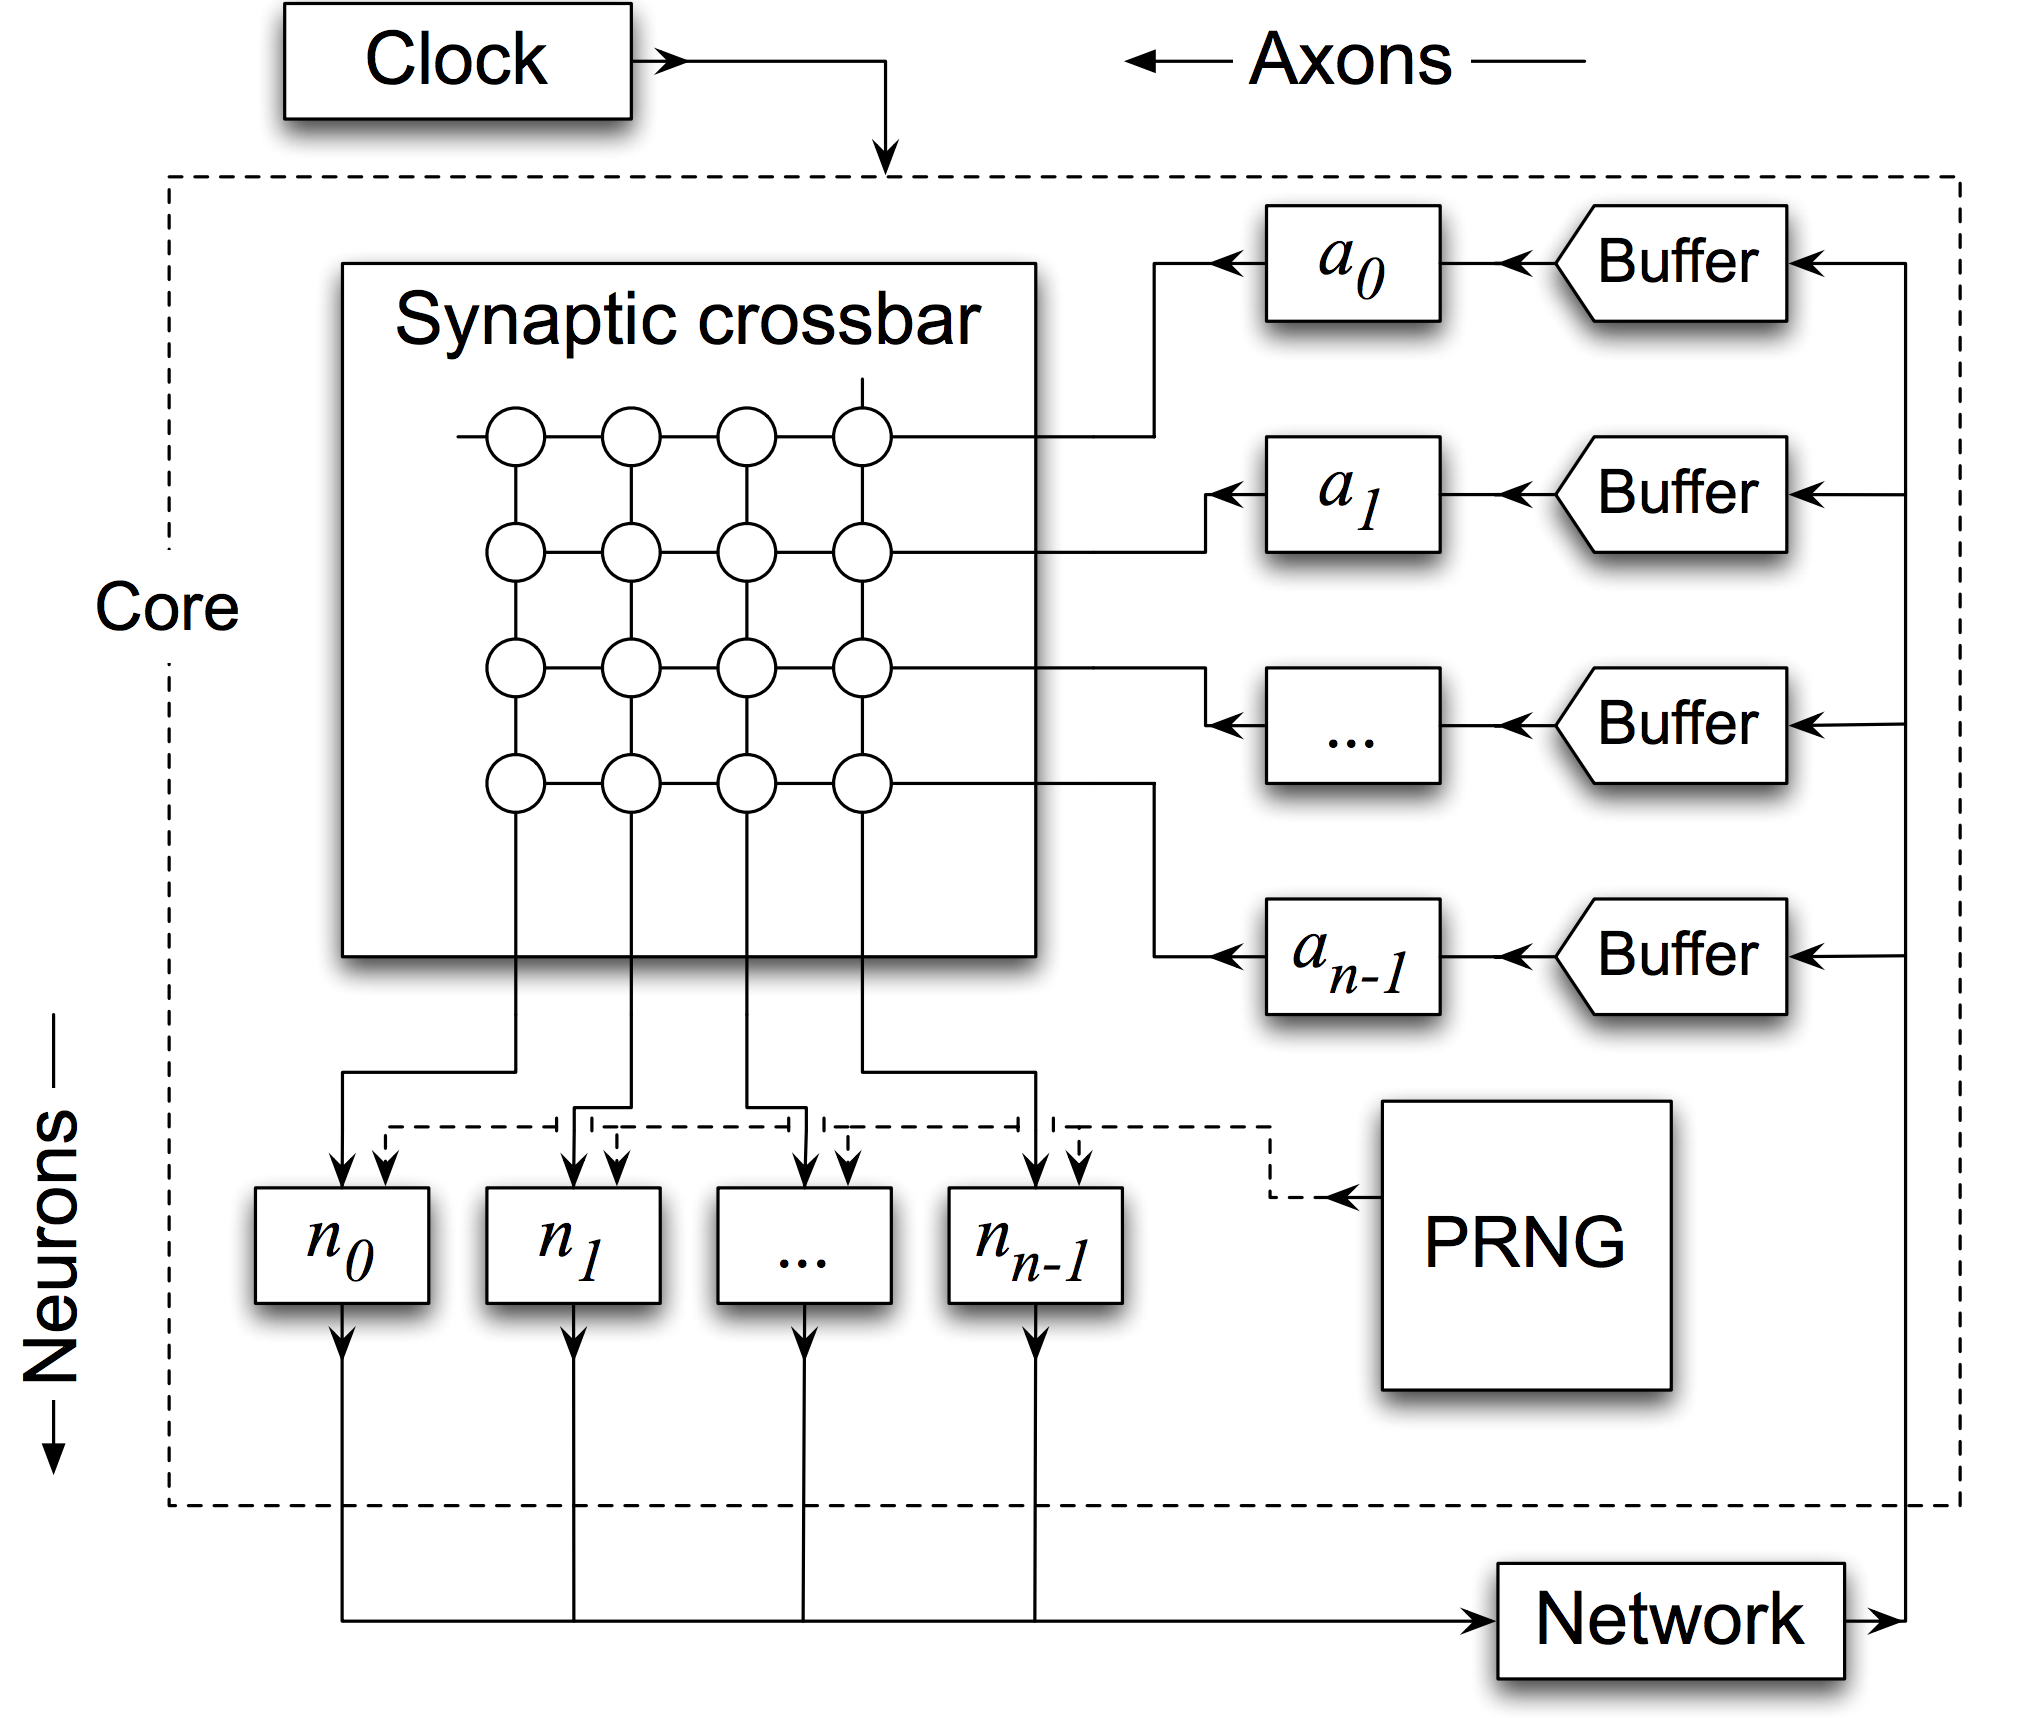
\includegraphics[width=0.6\linewidth]{fig/truenorth-arch}
  \caption{Conceptual architecture of a neurosynaptic core used in the TrueNorth
  chip. Reprint from \cite{Preissl2012}.}
  \label{fig:truenorth-arch}
\end{figure}

IBM has implemented an ecosystem of algorithms, libraries, simulators, a
programming language and an integrated development environment to support the
platform. Several applications for the chip has also been developed, such as a
multi-object detection and classification system operating on $240\times400$
pixel, 3-color video input at 30 frames per second.

\subsection{Tensor Processing Unit}

To accelerate training and utilization of machine learning models implemented
using their TensorFlow\footnote{\url{https://www.tensorflow.org/}}, Google have
designed an Application Specific Integrated Circuit (ASIC), the Tensor
Processing Unit (TPU)\cite{Jouppi2017}. Designed to provide exceptionally fast
matrix mutliplication, the TPU is built around a Matrix Multiply Unit (MMU)
capable of $2^{16}$ 8-bit multiply-and-add operations on signed/unsigned
integers per cycle. The rest of the logic on the chip is dedicated to moving and
organising data in such a way that the MMU is maximally utilized.

When compared with its contemporary CPU and GPU competitors, the TPU operates
approximately 15-30x faster, and with 30-80x higher TeraOps/Watt.

\begin{figure}[ht]
  \centering
  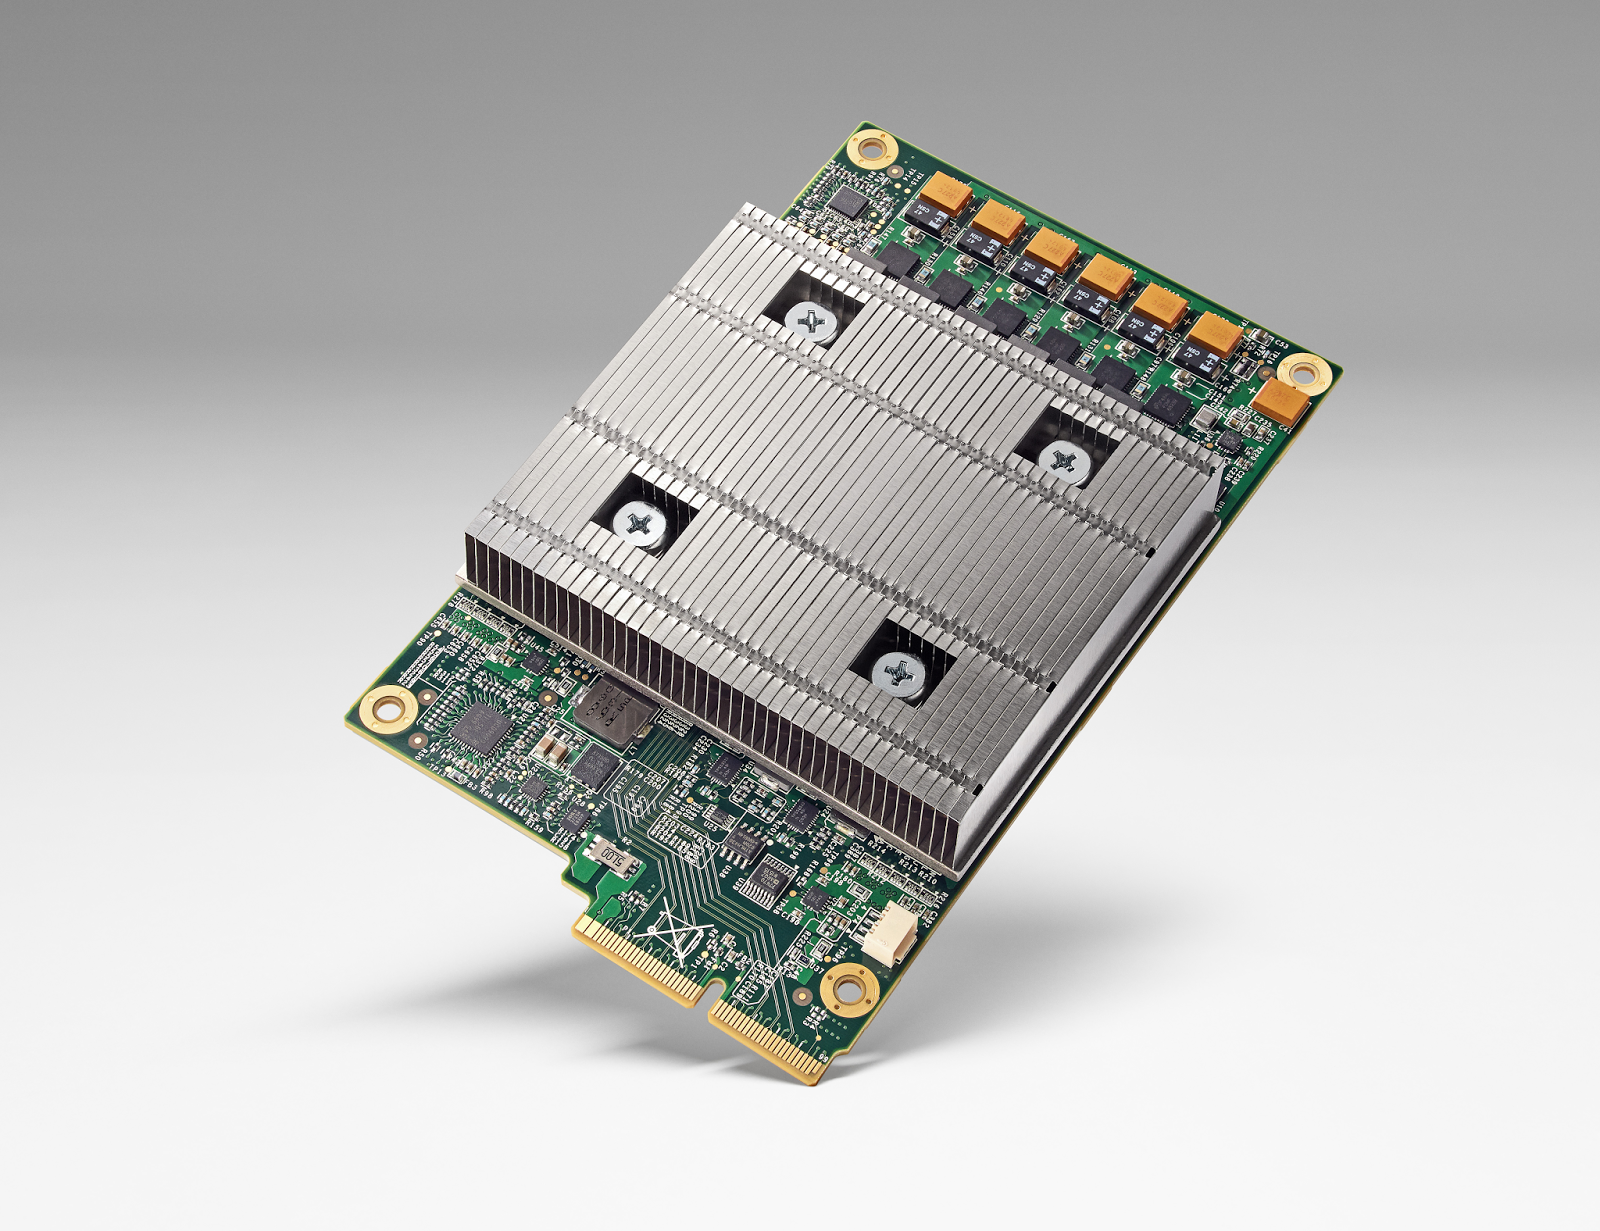
\includegraphics[width=0.8\linewidth]{fig/tpu-img}
  \caption[The Google Tensor Processing Unit]{The Google Tensor Processing Unit. Reprinted from \footnotemark}
  \label{fig:tpu-arch}
\end{figure}

\footnotetext{\href{https://cloudplatform.googleblog.com/2016/05/Google-supercharges-machine-learning-tasks-with-custom-chip.html}{\texttt{https://cloudplatform.googleblog.com}}}


\cleardoublepage
%%% Local Variables:
%%% mode: latex
%%% TeX-master: "../thesis"
%%% End:
